\documentclass{mcmthesis}
\mcmsetup{CTeX = false,    % 使用 CTeX 套装时,设置为 true
          tcn = {2520861}, problem = \textcolor{red}{C},
          sheet = true, titleinsheet = true, keywordsinsheet = true,
          titlepage = false, abstract = false}
        
\usepackage{newtxtext}     % \usepackage{palatino}
\usepackage[style=apa,backend=biber]{biblatex}
\addbibresource{reference.bib}

\usepackage{tocloft}
\usepackage{subcaption}

\usepackage{float}  %控制图片和表格的位置
\usepackage{indentfirst} %s首行缩进
\usepackage{threeparttable} %添加表格注释
\setlength{\cftbeforesecskip}{6pt}
%\setlength{\parindent}{2em} %全局首行缩进2字符
\renewcommand{\contentsname}{\hspace*{\fill}\Large\bfseries Contents \hspace*{\fill}}

\title{{\bf title}}
% \author{\small \href{http://www.latexstudio.net/}
%   {
\includegraphics[width=7cm]{mcmthesis-logo}}}
\date{\today}

\begin{document}
%%%%%%%%%%%%%%%%%%%%%%%%%%%%%%%%%%%%%%%摘要%%%%%%%%%%%%%%%%%%%%%%%%%%%%%%%%%%%%%%%%
\begin{abstract}

    During the 2024 Paris Summer Olympics, there was a surge in public interest in individual events and the medal rankings of various countries. Before each Olympic Games, a "virtual medal table" is created to predict the performance of different nations, but such predictions are typically based not only on historical medal data but also significantly influenced by the participating athletes. This article uses information such as the number and types of events a country participates in, project results, the host country, and specialty events to create a model.

    For issues one \& two, we used K-Means clustering to categorize the countries that have won medals into three types. We calculated the correlation between each country and different events using Pearson correlation coefficients, in order to identify the country's signature events. Based on these three types of countries, we applied the LSTM model for medal count training and prediction. Based on this model, we predicted the medal counts for each country in the 2028 Los Angeles Summer Olympics. The model also found that the number and types of Olympic events have a significant impact on a country's medal count.

    For issue three, we used a random forest algorithm to build a model for predicting countries that will win medals for the first time. The goal was to identify the key factors influencing the change in a country's medal count. We selected three feature variables: "number of participants," "number of participations," and "number of events," with "Will\_Earn\_Medal" as the target variable. We trained the model using a random forest regression model and used GridSearchCV to select the best hyperparameters, resulting in the optimal model configuration. We then calculated the probability of each country winning a medal. Finally, the model's performance was evaluated through confusion matrices and ROC curves, showing high prediction accuracy.

    For issue four, we used graph theory and network flow theory to quantitatively assess the influence of "great coaches" on a country's medal count. We established a directed network graph between coaches and countries, transforming the coach's impact on medals into node and edge flow relationships. The weight was calculated using the formula: $W=3\times \triangle G+2\times \triangle S+1\times \triangle B$. We then analyzed the coach's contribution to medals through total flow and bottleneck flow, providing an optimized path for countries in selecting coaches and helping them formulate more precise sports development strategies.
   
    For issue five, during the modeling process for the above issues, we identified some strategies that can help national Olympic committees increase their medal count. For example, with the increasing participation of women, national Olympic committees can focus on mixed-gender events to enhance winning opportunities. If a country is the host nation, it can apply to add domestic advantage events, optimize infrastructure, and increase financial support to leverage the home advantage and increase medal count. For events that are not monopolized by a few countries, strong nations should analyze these events and invest in cultivating the next generation of athletes, while emerging sports nations can achieve breakthroughs in these non-monopolized events by precisely targeting projects and bringing in excellent coaches.
    \begin{keywords}
        Prediction, LSTM, Random Forest, Olympic Games, Performance Modeling, Graph Theory
\end{keywords}
\end{abstract}


%%%%%%%%%%%%%%%%%%%%%%%%%%%%%%%%%%%%%%%目录%%%%%%%%%%%%%%%%%%%%%%%%%%%%%%%%%%%%%%%%
\maketitle

\tableofcontents
\thispagestyle{empty}

\newpage
%%%%%%%%%%%%%%%%%%%%%%%%%%%%%%%%%%%%%%%引言%%%%%%%%%%%%%%%%%%%%%%%%%%%%%%%%%%%%%%%%
\section{Introduction}
\hfill Faster, Higher, Stronger - Together.
\subsection{Background}%%%%%%%%背景
The Paris Olympics attracted global attention, with the events attracting a lot of attention, especially the medal results of the athletes from different countries. Athletes from all over the world fought hard to get a place on the medals table. In addition to the traditional Olympic powerhouses and the hosts' medal race attracting much attention, there was also much discussion about some of the lower-ranked countries, such as Albania, Cape Verde, Dominica and Saint Lucia, who won their first ever medals at the Paris Games. However, there are still more than 60 countries that have failed to collect Olympic medals.

Looking back at history, countries' medal performances in the Olympics show a certain pattern. Before each Olympics, there will be a ‘virtual medal table’ to predict the performance of countries. For example, before the Paris Olympics, Nielsen Gracenote released its final Virtual Medal Table (VMT) predictions for the 2024 Olympics. So what specific factors do such predictions rely on? The fact is that medal predictions are usually made near the start of the Olympic Games by building mathematical models that take into account known athlete participation plans and analysing past gold and total medal counts, in order to predict future medal rankings. Such forecasts are not only valuable to sports analysts, researchers and policymakers, but also help countries to better grasp the trends affecting Olympic performance.

\subsection{Restatement of the Problem}%%%%%%%%问题重述
Given the background information and constraints of the problem, we must complete the following tasks:
\begin{itemize}
\item Task 1: Predict the medal table for the 2028 Summer Olympics in Los Angeles, USA, outputting the countries that will perform better as well as those that will perform worse.
\item Task 2: Analyse the relationship between the number and type of Olympic sports and the number of medals, output the most important sports for each country and analyse the impact of the host country's choice of sports on performance.
\item Task 3: For countries that have not yet won a medal, predict the probability that they will win their first medal at the next Olympic Games and provide an estimate of the probability of this prediction
\item Task 4: Explore the impact of the Great Coach effect on team sports, looking for evidence of the impact of the Great Coach effect and estimating the strength of the effect. Finally, select three countries to recommend sports that are worth investing in and estimate their impact.
\item Task 5: Provide original insights into Olympic medal counts and explain how these insights inform the Olympic Committee's decision-making.
\end{itemize}

\subsection{Our Work}%%%%%%%%文章分析


%%%%%%%%%%%%%%%%%%%%%%%%%%%%%%%%%%%%%%%假设%%%%%%%%%%%%%%%%%%%%%%%%%%%%%%%%%%%%%%%%%%%
\section{Assumptions and Justification}

%%%%%%%%%%%%%%%%%%%%%%%%%%%%%%%%%%%%%%%符号说明%%%%%%%%%%%%%%%%%%%%%%%%%%%%%%%%%%%%%%%%
\section{Notations}

%%%%%%%%%%%%%%%%%%%%%%%%%%%%%%%%%%%%%%%数据处理%%%%%%%%%%%%%%%%%%%%%%%%%%%%%%%%%%%%%%%%
\section{Data Cleaning}
The study began with a systematic cleaning and pre-processing of the raw data.

In terms of athlete data processing, we performed operations such as removing duplicate entries, handling missing values, standardizing, and converting data types on the summerOly\_athletes.csv dataset, which contains basic athlete information (name, team, NOC, sport, events, medals, etc.). In addition, we found that the presence of spaces in the string text affected the subsequent data analyses, so we used str.strip() to remove leading and trailing spaces, and str.replace() to remove internal spaces. We also deleted invalid information and performed reverse processing on the summerOly\_programs.csv dataset for easier future use

In the NOC (National Olympic Committee) validation session, we used the athletes dataset as the primary reference source for valid NOCs and cross-validated it with the hosts and medals datasets. To ensure data consistency, we removed NOC entries from the hosts and medals datasets that were not present in the athletes dataset. This step provided a reliable foundation for subsequent data analyses.

To ensure data quality, we performed strict validation and quality checks, including ensuring consistency of NOC codes across all datasets, verifying year ranges and temporal continuity, and checking logical constraints such as the number of gold medals not exceeding the total number of medals. Care was taken to maintain the integrity of the data at all times during the dataset consolidation process.

Finally, we performed necessary additional transformations on the data, created an aggregated view of historical performance, unified the data format of each dataset, and prepared a standardised data structure for subsequent analysis and modelling. Through this series of rigorous data cleansing processes, we ensured the consistency, completeness and normality of the datasets, laying a solid foundation for the predictive modelling phase. These steps not only improve the data quality, but also enhance the reliability of the results of subsequent analyses.


%%%%%%%%%%%%%%%%%%%%%%%%%%%%%%%%%%%%%%%模型结构%%%%%%%%%%%%%%%%%%%%%%%%%%%%%%%%%%%%%%%%
\section{TASK1\&2: Medal Count Prediction Based on LSTM}

\subsection{Data Analysis}
First, we constructed a Feature Correlation Matrix for countries that have previously won medals to identify the advantage sports of some nations. Subsequently, we created contingency tables for each country, including features such as the year of medal wins, total medal count, gold medal count, host status, number of participants, number of events participated in, total events established by the host, and events from past editions. Finally, we used K-Means clustering to classify countries that have previously won medals into three categories, which serves as the basis for building separate predictive models for different types of Olympic nations.
\subsubsection{Correlation Matrix Analysis Based on Pearson Correlation}
\begin{itemize}
\item Step 1: Data Preparation:Align the medal count dataset with the event dataset to ensure that each row represents the number of medals a country won in a specific event.
\item Step 2: Pearson Correlation:The Pearson correlation coefficient is suitable for analyzing data that follows a continuous normal distribution. The calculation formula is as follows:

\begin{equation} \label{13}
    \rho(x,y)=\frac{\mathrm{cov}(x,y)}{\sigma(x)\cdot\sigma(y)}=\frac{E[(x-\mu_x)(y-\mu_y)]}{\sigma(x)\cdot\sigma(y)}
\end{equation}

\item Step 3: Correlation Calculation:For each country, we combined the number of medals won by that country in various events with the total number of medals awarded across different Olympic events to calculate the Pearson correlation coefficient. The Pearson correlation coefficient quantifies the strength of the relationship between variables. The intensity of variable correlations is shown in Figure [ ]. We visualized the resulting correlation matrix and, taking China as an example, generated a heatmap as shown in Table .

\begin{table}[H]
    \centering
    \caption{Variable Correlation Strength}
    \vspace{-0.3pt}
    \begin{tabularx}{\textwidth}{>{\centering\arraybackslash}X>{\centering\arraybackslash}X>{\centering\arraybackslash}X>{\centering\arraybackslash}X>{\centering\arraybackslash}X>{\centering\arraybackslash}X}
        \toprule[2pt]
        \textbf{Correlation Strength}  & \textbf{Very Strong Correlation}     & \textbf{Strong Correlation} & \textbf{Moderate Correlation} & \textbf{Weak Correlation} & \textbf{Very Weak or No Correlation} \\ 
        \midrule[1pt]
        \textbf{Absolute value of correlation coefficient} & \makebox[2cm]{0.8--1} & \makebox[2cm]{0.6--0.8} & \makebox[2cm]{0.4--0.6} & \makebox[2cm]{0.2--0.4} & \makebox[2cm]{0--0.2} \\ 
        \bottomrule[2pt]
    \end{tabularx}
    \label{tab:feature_importance}
\end{table}

\begin{figure}[htbp]
    \centering
    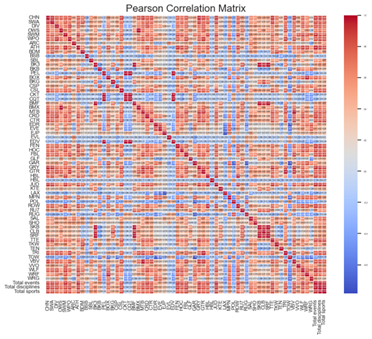
\includegraphics[width=12cm]{res/graph/heatmapofChina.png}
    \caption{Heatmap of China} \label{Figure 4}
\end{figure}

\end{itemize}








%%%%%%%%%%%%%%%%%%%%%%%%%%%%%%%%%%%%%%%敏感性分析%%%%%%%%%%%%%%%%%%%%%%%%%%%%%%%%%%%%%%%%




\end{document}